\documentclass{beamer}
\usepackage[utf8]{inputenc}
\usepackage[francais]{babel} 
\usepackage{graphicx} 
\usepackage{textcomp}
\usepackage{latexsym}
\usepackage{amssymb}
\usepackage{enumerate}
\usepackage{listings}
\usepackage{tikz}

\usetheme{Warsaw}

%\setbeamercolor{normal text}{fg=white,bg=black!90}
%\setbeamercolor{structure}{fg=white}
%
%\setbeamercolor{alerted text}{fg=red!85!black}
%
%\setbeamercolor{item projected}{use=item,fg=black,bg=item.fg!35}
%
%\setbeamercolor*{palette primary}{use=structure,fg=structure.fg}
%\setbeamercolor*{palette secondary}{use=structure,fg=structure.fg!95!black}
%\setbeamercolor*{palette tertiary}{use=structure,fg=structure.fg!90!black}
%\setbeamercolor*{palette quaternary}{use=structure,fg=structure.fg!95!black,bg=black!80}
%
%\setbeamercolor*{framesubtitle}{fg=white}
%
%\setbeamercolor*{block title}{parent=structure,bg=black!60}
%\setbeamercolor*{block body}{fg=black,bg=black!10}
%\setbeamercolor*{block title alerted}{parent=alerted text,bg=black!15}
%\setbeamercolor*{block title example}{parent=example text,bg=black!15}


\title{Smart Social Network - Projet de Master 2 SSI}

\author{
    Zakaria \textsc{Addi}
    Baptiste \textsc{Dolbeau}\\
    Yicheng \textsc{Gao}
    Florian \textsc{Guilbert}\\
    Giovanni \textsc{Huet}
    Emmanuel \textsc{Mocquet}\\
    Maxence \textsc{Péchoux}
    Romain \textsc{Pignard}
}
\institute{Université de Rouen}

\AtBeginSection[]
{
    \begin{frame}
        \tableofcontents[currentsection]
    \end{frame}
}

\begin{document}

\begin{frame}
\titlepage 
\end{frame}

\begin{frame}
\frametitle{Plan}
\tableofcontents%[hideallsubsections]
\end{frame}

\section{Introduction}

\section{Carte à puce}

\subsection{Présentation}
\begin{frame}
    \frametitle{Présentation}
    \begin{block}{}
    \end{block}
\end{frame}


\subsection{Les besoins}
\begin{frame}
    \frametitle{Les besoins}
    \begin{block}{}
    \end{block}
\end{frame}

\subsection{Côté carte : SmartCard }
\begin{frame}
    \frametitle{Côté carte : SmartCard}
    \begin{block}{}
    \end{block}
\end{frame}

\subsection{Côté client : GeneralClient}
\begin{frame}
    \frametitle{Côté client : GeneralClient}
    \begin{block}{}
    \end{block}
\end{frame}

\subsection{Démonstration}
\begin{frame}
    \frametitle{Démonstration}
    \begin{block}{}
    \end{block}
\end{frame}

\subsection{L'interface avec SSN : SoftCard}
\begin{frame}
    \frametitle{L'interface avec SSN : SoftCard}
    \begin{block}{}
    \end{block}
\end{frame}

\subsection{Quid de la sécurité ?}
\begin{frame}
    \frametitle{Quid de la sécurité ?}
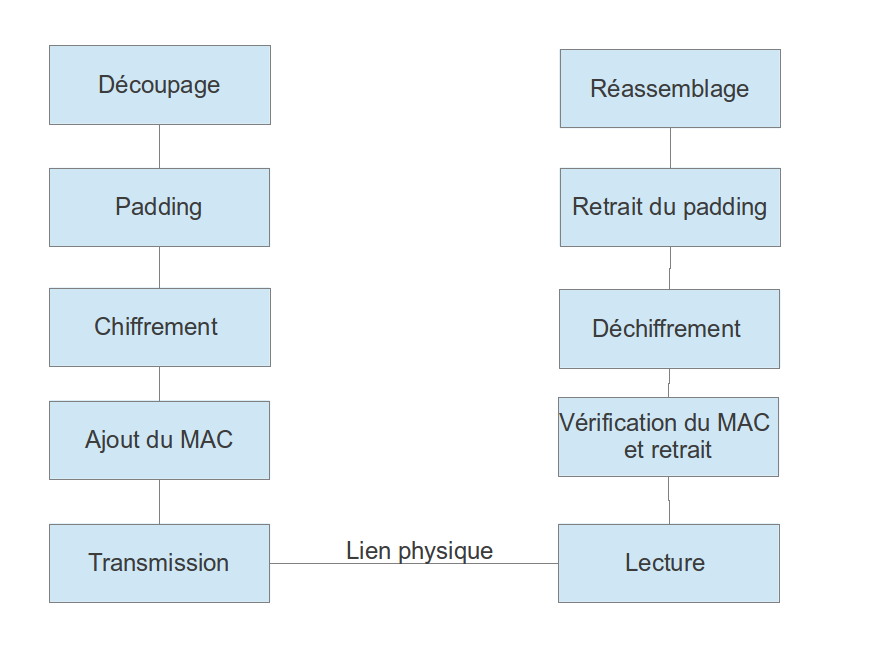
\includegraphics[width=9cm]{stack}

    \begin{block}{}
    \end{block}
\end{frame}

\section{Une protection vis-à-vis de Facebook}

\subsection{Présentation}

\begin{frame}
    \frametitle{Présentation}
    \begin{block}{ }
    \end{block}
\end{frame}





\end{document}
